

\section{Experiments}\label{sec:experiments}
\begin{figure*}[t]
    \centering
    \centerline{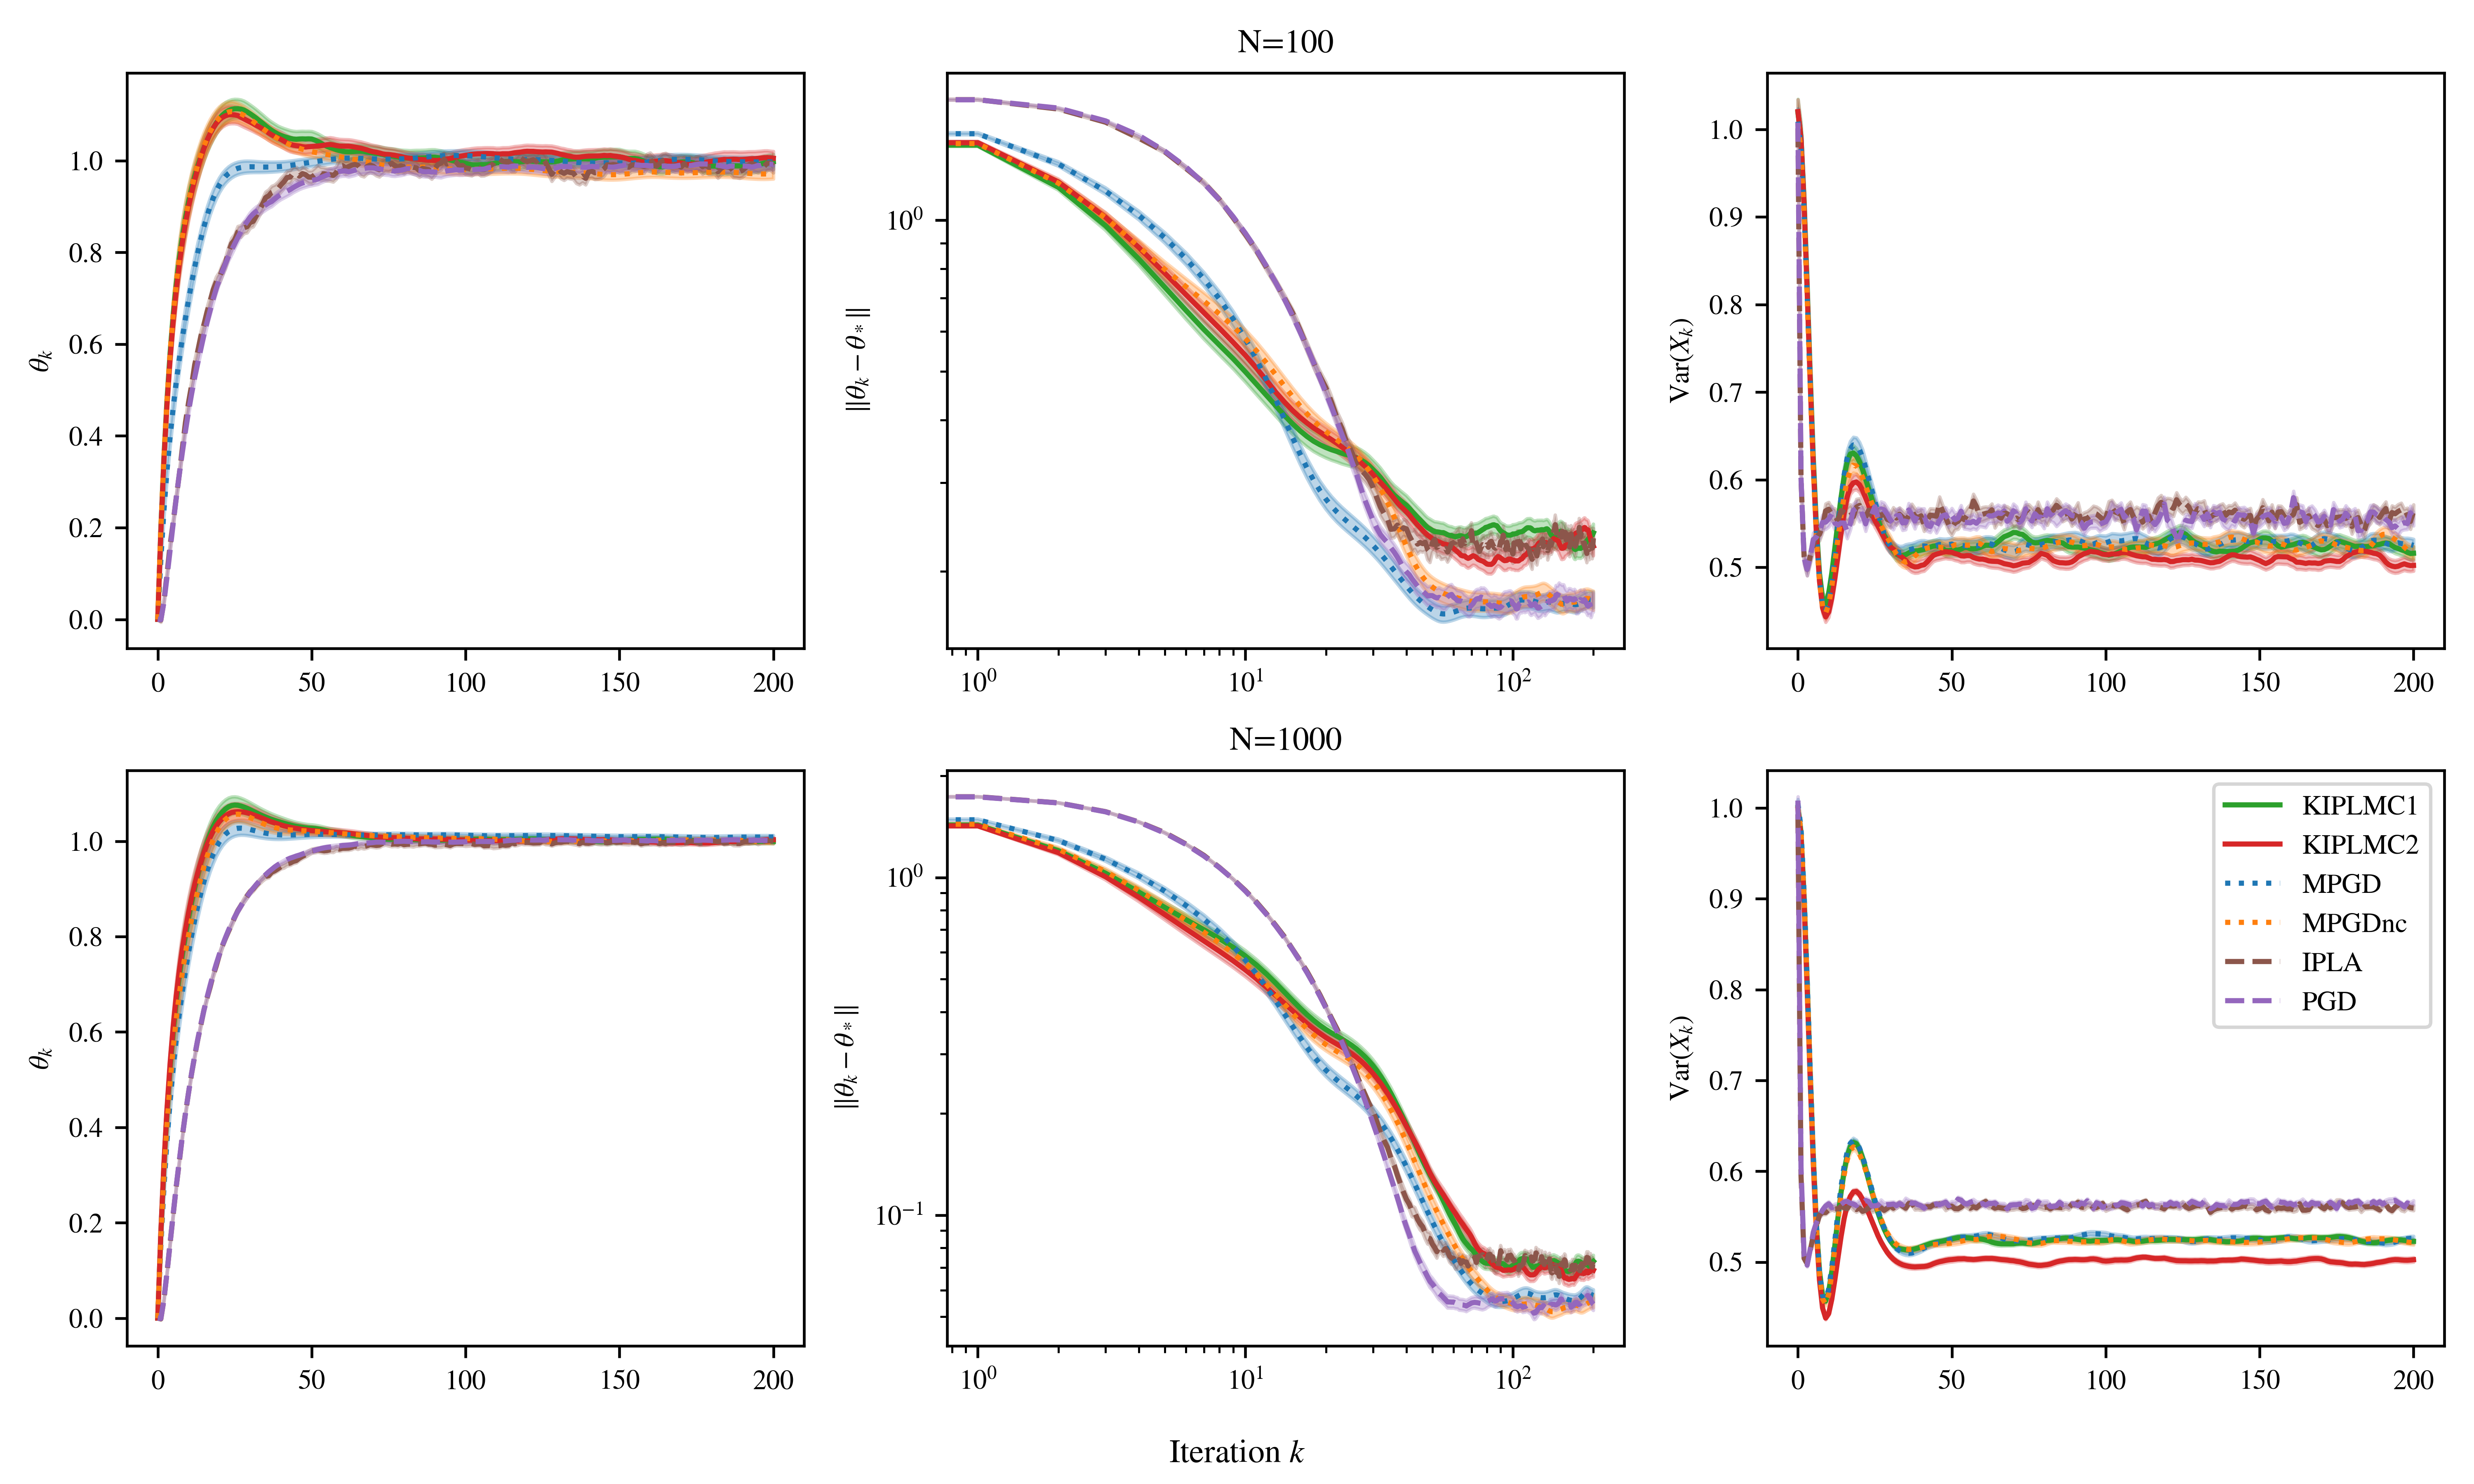
\includegraphics[width=\textwidth]{plots/fig1.png}}
    \caption{\textbf{Parameter estimate comparison.} We compare the performance of the \gls*{pgd}, \gls*{ipla}, \gls*{mpgd}, \gls*{kiplmc1}, and \gls*{kiplmc2} algorithms on the synthetic dataset with true $\bar{\theta}_\star = \mathbbm{1}_{d_x}$. We observe the desired convergence of behaviours for larger values of $N$ in the parameter space, mean-square error and the posterior variance of $X_k^i$. In this example $d_x=d_\theta=3$, $d_y=100$ and $\gamma=2.2$. Here we choose $\theta_0, X_0^i, V^\theta_0, V^{x_i}_0\sim\mathcal{N}(0, 0.1)$ and run 100 Monte Carlo simulations.}
    \label{fig:pgdcomparison}
\end{figure*}
In the following section a comparison will be made between the empirical results of \gls*{kiplmc1}, \gls*{kiplmc2} algorithms, as well as, those of \gls*{pgd} from \citep{kuntz2023particle}, \gls*{ipla} from \citep{akyildiz2025interacting} and \gls*{mpgd} from \citep{lim2023momentum}. We note that, in \citep{lim2023momentum}, the \gls*{mpgd} is not solely the discretisation of the KIPLD-like \gls*{sde} using the exponential integrator, but includes a \textit{gradient correction} term, making theoretical analysis and a direct comparison with our methods non-trivial (for a comparison of computational cost see Sec.~\ref{app:compcost}). To this end, we will also compare these methods to MPGDnc, the \gls*{mpgd} algorithm implemented without gradient correction, so that the number of gradient computations is the same as \gls*{kiplmc1}.

In the following sections, we will consider three examples: (i) Bayesian logistic regression on a synthetic dataset, (ii) Bayesian logistic regression on the Wisconsin Cancer dataset, and (iii) a \gls*{bnn} example as a more challenging, non-convex example on the MNIST dataset.

\begin{figure*}[h]
    \centering
    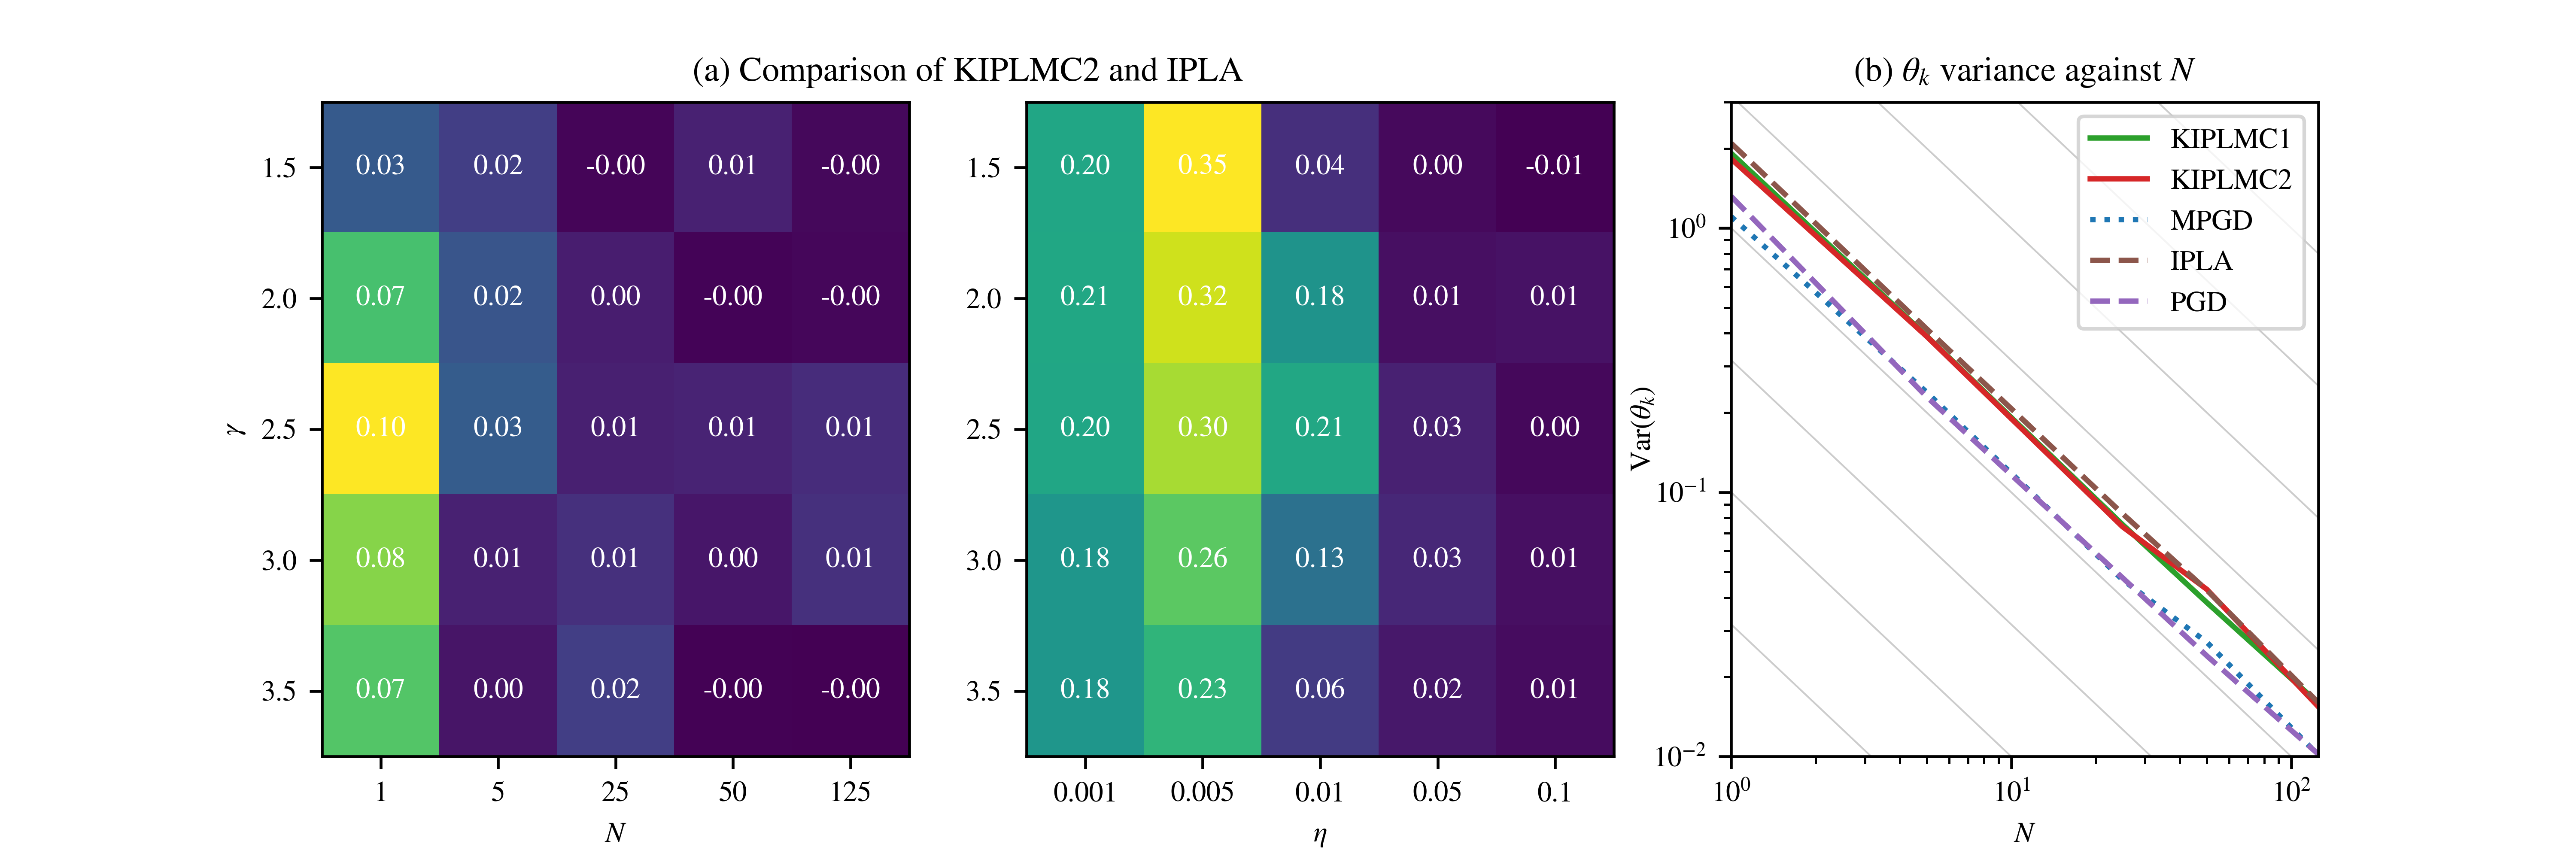
\includegraphics[width=\linewidth]{plots/fig2.png}
    \caption{\textbf{Comparison over hyper-parameters.} (a) shows the Area Between the Curves (ABC) values between \gls*{ipla} and \gls*{kiplmc2} for a variety of hyper-parameter combinations. The larger the positive value, the greater the acceleration of \gls*{kiplmc2} with respect to \gls*{ipla} (discussed in C.1). (b) makes a comparison over 100 Monte Carlo simulations of the algorithms' sample variances, using the last 100 steps of each simulation. The grid-lines corresponding to $1/N$ are provided to highlight the rate of convergence. Where not specified otherwise, simulations are run with $M=2000$, $\eta=0.005$, $\gamma=2.2$ and $N=100$.}
    \label{fig:convergence_var}
\end{figure*}

\subsection{Bayesian Logistic Regression on Synthetic Data}\label{sec:toyex}
We follow the experimental setting in \citep{kuntz2023particle} and \citep{akyildiz2025interacting} and start with comparisons between algorithms on a synthetic dataset for which we know the true solution. More precisely, consider the Bayesian logistic regression model
\begin{align*}
p_\theta(x) &= \mathcal{N}(x; \theta, \sigma^2 I_{d_x})\\
p(y|x) &= \prod_{j=1}^{d_y} s(v_j^\intercal x)^{y_j} (1-s(v_j^\intercal x))^{1-y_j}.
\end{align*}
Here $s(u)=e^u/(1+e^u)$ is the logistic function and $v_j$, $j\in[d_y]$ are the set of $d_x$-dimensional covariates with corresponding responses $y_j\in\{0,1\}$. $\sigma$ is given and fixed throughout. We generate a synthetic set of covariates, $\{v_j\}_{j=1}^{d_y}\subset \mathbb{R}^{d_x}$, from which are simulated a synthetic set of observations $y_j|\bar{\theta}_\star, x, v_j$, for fixed $\bar{\theta}_\star$, via a Bernoulli random variable with probability $s(v_j^\intercal x)$. The algorithm is tested on the recovery of this value of $\bar{\theta}_\star$. 

The marginal likelihood is given as,
\begin{align*}
&p_\theta (y)\\
&= \int \left(\prod_{j=1}^{d_y} s(v_j^\intercal x)^{y_j} (1-s(v_j^\intercal x))^{1-y_j} \right) p_\theta(x)\mathrm{d}x.
\end{align*}
From this it easy to see that the gradients of $U$ are given as,
\begin{equation}\label{eq:logreggrad}
\begin{aligned}
 \nabla_\theta U(\theta, x) &= -\frac{x-\theta}{\sigma^2},\\
 \nabla_x U(\theta,x) &= \frac{x-\theta}{\sigma^2} - \sum_{j=1}^{d_y} (y_j - s(v_j^\intercal x))v_j.   
\end{aligned}
\end{equation}

\begin{remark}[On \ref{assump:strongconvexity} and \ref{assump:lipschitz}]\label{rem:convexity}

We will discuss this problem and our assumptions. Writing $z=(\theta,x)$ and $z'=(\theta',x')$, using
$\|(a-b,-a+b)\|\leq2\|(a,b)\|$ and the fact that the logistic function is $1/4$-Lipschitz, we obtain
\begin{equation*}
\begin{aligned}
\|\nabla U(z)-\nabla U(z')\|
&\leq\left(\frac{2}{\sigma^2}+\frac14\sum_{j=1}^{d_y}\|v_j\|^2\right)\|z-z'\|.
\end{aligned}
\end{equation*}
Hence, \ref{assump:lipschitz} is satisfied \citep{akyildiz2025interacting}.

For \ref{assump:strongconvexity}, note that $d_\theta=d_x$ in this model. Set
$q_j(x):=s(v_j^\intercal x)\bigl(1-s(v_j^\intercal x)\bigr)$ and
$Q(x):=\sum_{j=1}^{d_y}q_j(x)v_jv_j^\intercal$. Then
\begin{equation*}
\begin{aligned}
\nabla^2U(z)
&=\frac1{\sigma^2}
\begin{pmatrix}
I_{d_x}&-I_{d_x}\\
-I_{d_x}&I_{d_x}
\end{pmatrix} +\begin{pmatrix}
0&0\\
0&Q(x)
\end{pmatrix}.
\end{aligned}
\end{equation*}
Indeed, for $u,w\in\mathbb R^{d_x}$, $(u, w)^\intercal\nabla^2U(z)(u,w)$ vanishes if and only if $u=w$ and $v_j^\intercal w=0$ for every $j$.
Thus, $U$ is strictly convex provided that
$\operatorname{span}\{v_1,\ldots,v_{d_y}\}=\mathbb R^{d_x}$. Consequently, \ref{assump:strongconvexity} is not satisfied without further regularisation; nevertheless, we believe that this remains a useful illustrative example.
\end{remark}

In Fig.~\ref{fig:pgdcomparison} we can see the difference in the behaviours between the algorithms. Most notably, the \gls*{kiplmc1} and \gls*{kiplmc2} algorithms exhibit comparable levels of acceleration as the \gls*{mpgd} algorithm in the $\theta$-dimension, whilst the \gls*{ipla} and \gls*{pgd} algorithms trail further behind. Interestingly, we observe (more notably for large $N$) that the noise in the $\theta$-dynamics in \gls*{kiplmc1} and \gls*{kiplmc2}, as compared to \gls*{mpgd}, seems to dampen some of the momentum effects when $\gamma$, the friction coefficient is sub-optimal. As $N$ grows the $\theta$ iterates concentrate onto the \gls*{mmle} $\bar{\theta}_\star$ for all algorithms. This behaviour can be seen in more detail in Fig.~\ref{fig:convergence_var} (b), in which we can verify the variance changing with rate $\mathcal{O}(1/N)$. Further, we make a comparison of the performance of the \gls*{ipla} and \gls*{kiplmc2} in Fig.~\ref{fig:convergence_var} (a) with the Area Between the Curves (ABC) metric (see \ref{sec:ABC} for more detail). This metric is a signed, weighted difference between the performances of the two algorithms: the higher the value, the better \gls*{kiplmc2} performs compared to \gls*{ipla}; 0 is when they perform the same. We observe that the acceleration of \gls*{kiplmc2} can be best observed in specific $\gamma$ regimes, which ensure that the momentum is close to critical dampening.

Note that the momentum effects of the \gls*{kiplmc1} and \gls*{kiplmc2} algorithms has been dampened through a specific choice of $\gamma$. In training it was observed that the convergence rate is very sensitive to the choice of $\gamma$, where choices too small, exhibit large momentum effects, and too large, lead to slow convergence (see also \citep{lim2023momentum} for more discussion on the role of the momentum parameter for learning with KLMC). The choice of $\gamma$ here is far from optimal, but allows us to observe the strength of the proposed algorithms.

\begin{figure*}[b!]
    \centering
    \centerline{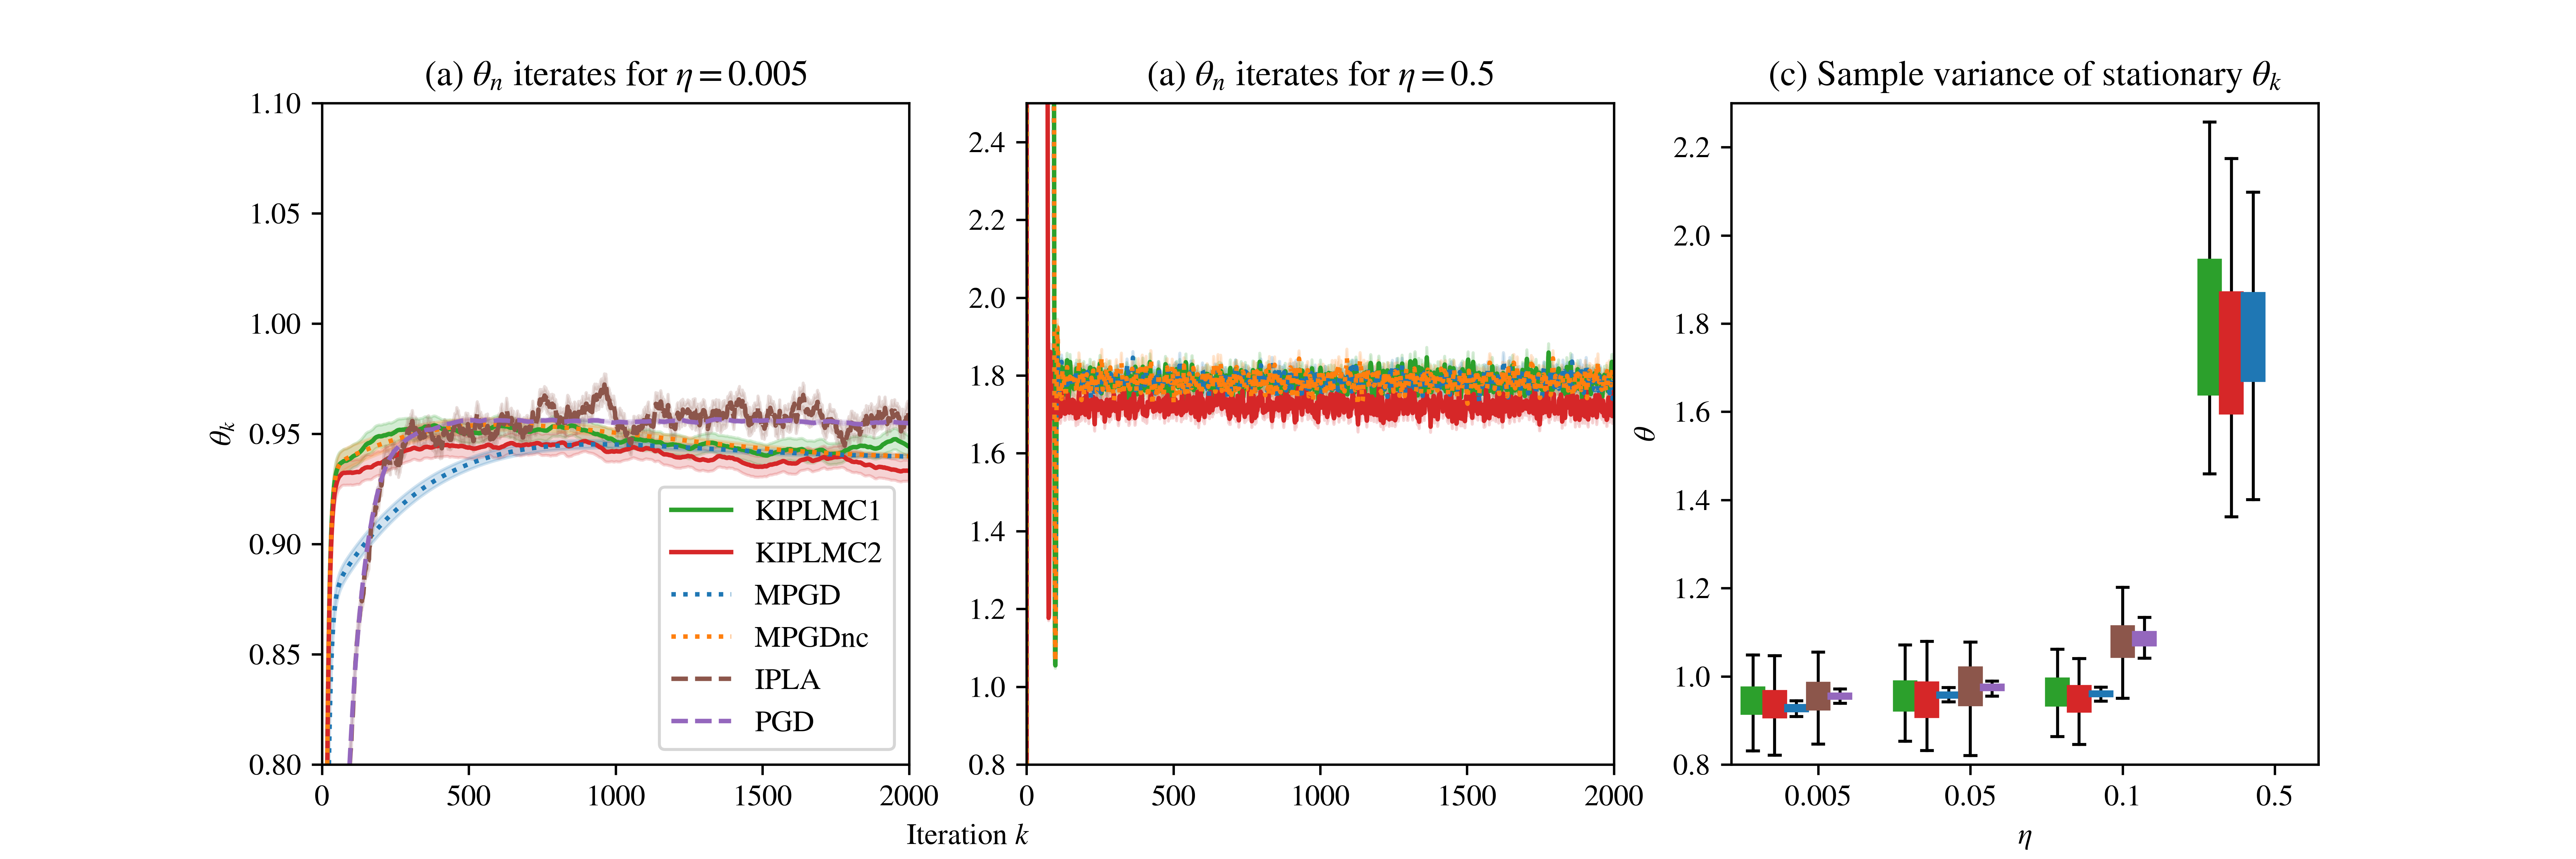
\includegraphics[width=\linewidth]{plots/fig3.png}}
    \caption{\textbf{Wisconsin Dataset.} The performance of \gls*{pgd}, \gls*{ipla}, \gls*{mpgd}, \gls*{kiplmc1} and \gls*{kiplmc2} algorithms are compared on a logistic regression experiment for the Wisconsin Cancer Dataset. In (a), we show the behaviour of the $\theta_n$ iterates for a small step-size and (b) shows the behaviour $\theta_n$ iterates for a step-size where \gls*{ipla} and \gls*{pgd} explode. In (c) we compare the distributions of the algorithms over different step-sizes. We set $N=100$ and $\gamma=3.2$.}
    \label{fig:wisconsin}
\end{figure*}

\subsection{Wisconsin Cancer Data}
\label{sec:cancex}

We follow again an experimental procedure that is similar to the one outlined in \citep{kuntz2023particle} and \citep{akyildiz2025interacting} and make comparisons between the algorithms on a more realistic dataset: the Wisconsin Cancer Data. Again, we use the logistic regression LVM model, outlined above. This task is a binary classification, to determine from 9 features gathered from tumours and 683 data points labelled as either benign or malignant. The latent variables correspond to the features extracted from the data. The task in this case is to seek to model the behaviour as accurately as possible through the logistic regression LVM.

For this setup we define our probability model as,
\begin{equation*}
p_\theta(x) = \mathcal{N}(x;\theta \mathbbm{1}_{d_x}, 5 I_{d_x})
\end{equation*}
and the likelihood as,
\begin{equation*}
p(y|x)=\prod_{j=1}^{d_y} s(v_j^\intercal x)^{y_j}(1-s(v_j^\intercal x))^{1-y_j}.
\end{equation*}
Note that the parameter $\theta$ is a scalar in this case, hence, this turns out to be a simplified version of the setup described above and so the discussion in Remark~\ref{rem:convexity} is still valid. As opposed to the previous case with synthetic data, here we consider a real dataset, so no ground-truth $\bar{\theta}^\star$ is available. Hence, there is no comparison to a $\bar{\theta}_\star$, but we can see that different algorithms attain similar estimates of this maximiser.

\begin{figure*}[t!]
    \centering
    \centerline{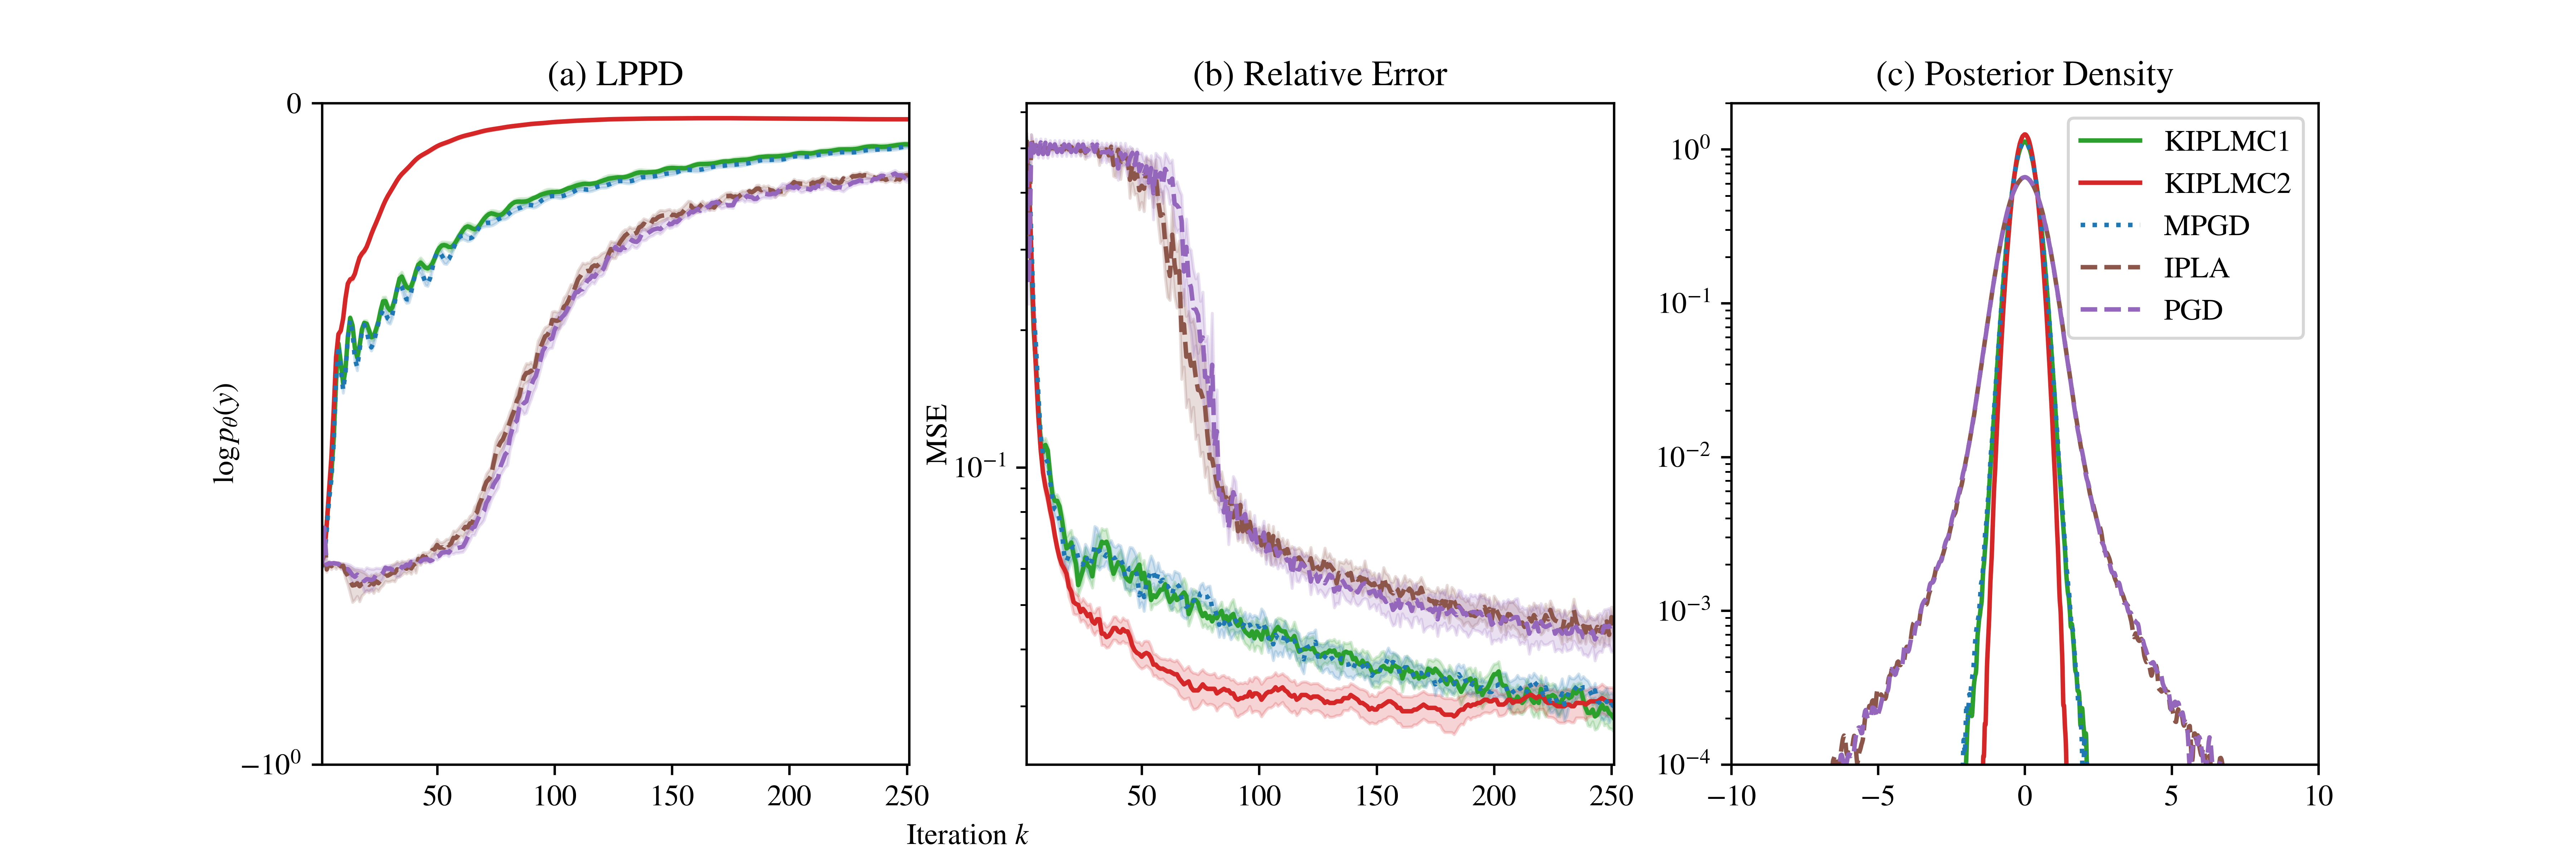
\includegraphics[width=\linewidth]{plots/fig4.png}}
    \caption{\textbf{MNIST Dataset.} The performance of \gls*{pgd}, \gls*{ipla}, \gls*{mpgd}, \gls*{kiplmc1} and \gls*{kiplmc2} algorithms are compared on a classification experiment for the MNIST Dataset. (a) shows the Log Pointwise Predictive Density, the average log probability assigned to the correct response. (b) shows the percentage error and (c) the posterior density of the weights $w$. For this experiment $N=100$, $\gamma=2$ and $\eta=0.01$.}
    \label{fig:bnn}
\end{figure*}

Most notably in this experiment, we can observe in Fig.~\ref{fig:wisconsin} the importance of the added stability that the momentum-based algorithms exhibit, with the use of more stable numerical integrators than Euler-Maruyama. In particular, these algorithms displays great stability w.r.t. the choice of the step-size, as well as, the acceleration one would expect. For small step-sizes, the \gls*{pgd} algorithm performs with low variance in all cases where it converges, until it explodes where step-sizes become too large . It is interesting to note however that in the large step-size regime, the momentum-based algorithms exhibit much greater momentum than in the smaller step-sizes. However, again, we note that the \gls*{kiplmc1} and \gls*{kiplmc2} algorithms exhibit more variance in the $\theta$ estimation than the \gls*{pgd} and \gls*{mpgd} algorithms, though it is damped when compared to the \gls*{ipla} algorithm, due to the higher regularity of the solutions to KIPLD. This is typically an advantage when working with convex problems, but this ``sticky'' behaviour might prove detrimental in the non-convex case \citep{gao2022global, akyildiz2025interacting}. The injection of noise into the parameter estimation may help the method to escape local minima \citep{akyildiz2024nonasymptotic}.


\subsection{Bayesian Neural Network}\label{sec:bnn}
Similarly to \citep{kuntz2023particle, lim2023momentum} we also consider a Bayesian Neural Network (BNN) example to perform character classification on the MNIST dataset. In this case our approach is similar to ``cold'' posterior estimation, as our sampling density is proportional to a density raised to the inverse temperature, as in \citep{coldposterior}.

This dataset and model provide a more challenging problem for the \gls*{kiplmc1} and \gls*{kiplmc2} algorithms as the posteriors are known to be multi-modal and hence do not satisfy assumption \ref{assump:strongconvexity}. Indeed, we consider this example for illustrative purposes, showing the relative strength of our proposed methods compared to similar \gls*{ips} methods in a non-convex setting. MNIST contains 70'000 $28\times 28$ grey-scale images $\{f_i\}_{i=1}^{70000} \subset \mathbb{R}^{784}$. However, to avoid issues of high dimensionality, we consider a normalised subset of 1,000 characters containing only images of fours and nines, whose similarity should pose a challenge. Due to this smaller sample, we are also able to avoid the need for sub-sampling.

Following \citep{kuntz2023particle} we employ a two layer BNN with $\tanh$ activation function, softmax output layer and 40 dimensional latent space. i.e. we consider the probability of the data labels $l$ to be conditionally independent, given the features $f$ and the weights $x=(w,v)$, with model,
\begin{equation*}
p(l|f, x) \propto \exp\left(\sum_{j=1}^{40} v_{lj} \tanh\left(\sum_{i=1}^{784} w_{ji} f_i\right)\right),    
\end{equation*}
where $w\in \mathbb{R}^{40\times 784}$, $v\in\mathbb{R}^{2\times 40}$. The model has no bias terms and we place the following Gaussian priors on the weights: $w\sim \mathcal{N}(0, e^{2\alpha}\mathbb{I})$ and $v\sim \mathcal{N}(0, e^{2\beta}\mathbb{I})$. Rather than assigning these priors, we learn the parameters $\theta=(\alpha, \beta)\in\mathbb{R}^2$ jointly with the latent variables $x$. Hence, the model's density is given as
\small
\begin{align*}
p_\theta(x, \{l\}_{i=1}^{1000} |\{f_i\}_{i=1}^{1000})= \mathcal{N}(w; 0,e^{2\alpha}) \mathcal{N}(v; 0, e^{2\beta})\prod_{i=1}^{1000} p(l_i|f_i, x).
\end{align*}
\normalsize
We will employ autograd methods from the PyTorch library to compute the gradients.

In Fig.~\ref{fig:bnn} we make a comparison between the different algorithms over 100 runs, comparing the log predictive point-wise density (LPPD) and relative error. The LPPD is the average log-likelihood assigned to the correct response, whilst the relative error is given as the accuracy of prediction on a test set (see \ref{sec:err} for more detail). Observe the improved behaviour of the momentum-based algorithms in LPPD, as well as relative error. We also note the significant acceleration observed for \gls*{kiplmc2}, highlighting the effect of the distinct numerical integrators. Similarly, in Fig.~\ref{fig:bnn} (c) we can see the more concentrated posterior distributions of the momentum-based algorithms. Thus, it is clear that the \gls*{kiplmc1} and \gls*{kiplmc2} algorithms perform competitively against other particle-based methods, even in very complex problems, in which our assumptions may not be satisfied.

\section{Conclusions}
This paper extends a line of work on interacting particle-, and more generally, diffusion-based algorithms for maximum marginal likelihood estimation. This paper has focused on alternatives to the \glspl*{ips} proposed by \citep{kuntz2023particle, akyildiz2025interacting, lim2023momentum} for the \gls*{mmle} problem by considering an accelerated variant. We have shown that we can leverage the existing literature on underdamped Langevin diffusion for sampling \citep{dalalyan2018sampling, cheng2018underdamped, monmarche2021high, Nesterovacc} to produce two algorithms with greater stability, added smoothness and exponential convergence, which concentrate onto the \gls*{mmle} with quantitative nonasymptotic bounds on the estimation error $\bE[\|\theta_n - \bar{\theta}_\star\|^2]^{1/2}$. In particular, we show that \gls*{kiplmc1} attains an accelerated error rate for error $\varepsilon$ after $\widetilde{\mathcal{O}}(\sqrt{d_x} \varepsilon^{-1})$ steps, compared to the \gls*{ipla} and \gls*{pgd} which require $\widetilde{\mathcal{O}}(d_x \varepsilon^{-2})$ steps. The proposed algorithms both perform well empirically compared to the \gls*{mpgd} and other particle methods. Specifically, the induced noise should improve guarantees in the non-convex setting, as discussed in \citep{akyildiz2025interacting, raginsky2017non,akyildiz2024nonasymptotic}. 

The results presented here hold under assumptions of gradient-Lipschitzness and strong log-concavity, however, it is possible to extend this line of work to the non-convex, super-linear or even proximal cases (for examples of this see, \citep{zhang2023nonasymptotic,akyildiz2024nonasymptotic,johnston2023kinetic, encinar2025proximal}). Another interesting direction is to consider the setting in \citep{fan2023gradient}, using an accelerated algorithm for high-dimensional linear models. Our methods can also be adapted to solving linear inverse problems as done by \citep{akyildiz2022statistical,glyn2024statistical}. Similar ideas can be considered within the setting of Stein variational gradient descent as done in \citep{sharrock2024tuning}. Crucially, the procedure used to obtain the bounds for the algorithms presented here can easily be extended to other cases, creating a powerful theoretical framework for further underdamped Langevin sampling algorithms for the \gls*{mmle} problem.
